% !TEX program = xelatex

\documentclass[hyperref, UTF8,11pt,a4paper]{ctexart} %只有10,11,12磅三个选项
\usepackage[utf8]{inputenc}
\usepackage{amsmath}
\usepackage{amsfonts}
\usepackage{amssymb}
\usepackage{float} % 图像浮动
\usepackage[xetex]{graphicx} % xetex驱动
\usepackage[left=1.00cm, right=0.50cm, top=0.20cm, bottom=0.20cm]{geometry}
\usepackage{color} % 颜色
\newcommand{\tabincell}[2]{\begin{tabular}{@{}#1@{}}#2\end{tabular}}
\title{数学笔记}	% 标题
\author{于洋}			% 作者
\date{}					% 日期
\linespread{1.5}	%行间距
% \renewcommand\arraystretch{1.3} %表格行高
\usepackage[breaklinks,colorlinks,linkcolor=black,citecolor=black,urlcolor=black]{hyperref} % 生成书签
\setlength{\parindent}{0pt}  % 设置缩进
\begin{document}
\tableofcontents
\maketitle

\newpage

%=========== [ 三角函数 ] =======================================
\section{三角函数}

%=========== 基础知识 ===========================================

\subsection{基础知识}
诱导公式:
\begin{figure}[!h] %figure参数:h 此处(here)t 页顶(top)b 页底(bottom)p 独立一页(page)
	\centering
	\begin{minipage}{170pt}
		$$
			\begin{array}{l}{\sin (2 k \pi+\alpha)=\sin \alpha, k \in \mathbb{Z}} \\ {\cos (2 k \pi+\alpha)=\cos \alpha, k \in \mathbb{Z}} \\ {\tan (2 k \pi+\alpha)=\tan \alpha, k \in \mathbb{Z}}\end{array}
		$$
	\end{minipage}
	\hspace{10pt}
	\begin{minipage}{170pt}
		$$
			\begin{array}{c}{\sin (\pi+\alpha)=-\sin \alpha} \\ {\cos (\pi+\alpha)=-\cos \alpha} \\ {\tan (\pi+\alpha)=\tan \alpha}\end{array}
		$$
	\end{minipage}
	\hspace{10pt}
	\begin{minipage}{170pt}
		$$
			\begin{array}{c}{\sin (-\alpha)=-\sin \alpha} \\ {\cos (-\alpha)=\cos \alpha} \\ {\tan (-\alpha)=-\tan \alpha}\end{array}
		$$
	\end{minipage}
\end{figure}
\begin{figure}[!h] %figure参数:h 此处(here)t 页顶(top)b 页底(bottom)p 独立一页(page)
	\centering
	\begin{minipage}{170pt}
		$$
			\begin{aligned} \sin (\pi-\alpha) &=\sin \alpha \\ \cos (\pi-\alpha) &=-\cos \alpha \\ \tan (\pi-\alpha) &=-\tan \alpha \end{aligned}
		$$
	\end{minipage}
	\hspace{10pt}
	\begin{minipage}{170pt}
		$$
			\begin{aligned} \sin \left(\frac{\pi}{2}+\alpha\right) &=\cos \alpha \\ \cos \left(\frac{\pi}{2}+\alpha\right) &=-\sin \alpha \\ \tan \left(\frac{\pi}{2}+\alpha\right) &=-\cot \alpha \end{aligned}
		$$
	\end{minipage}
	\hspace{10pt}
	\begin{minipage}{170pt}
		$$
			\begin{aligned} \sin \left(\frac{\pi}{2}-\alpha\right) &=\cos \alpha \\ \cos \left(\frac{\pi}{2}-\alpha\right) &=\sin \alpha \\ \tan \left(\frac{\pi}{2}-\alpha\right) &=\cot \alpha \end{aligned}
		$$
	\end{minipage}
\end{figure}
\\
两角和差:
\begin{figure}[!h] %figure参数:h 此处(here)t 页顶(top)b 页底(bottom)p 独立一页(page)
	\centering
	\begin{minipage}{170pt}
		$$
			\begin{aligned} \sin (\alpha+\beta) &=\sin \alpha \cos \beta+\cos \alpha \sin \beta \\ \sin (\alpha-\beta) &=\sin \alpha \cos \beta-\cos \alpha \sin \beta \\ \cos (\alpha+\beta) &=\cos \alpha \cos \beta-\sin \alpha \sin \beta \\ \cos (\alpha-\beta) &=\cos \alpha \cos \beta+\sin \alpha \sin \beta \end{aligned}
		$$
	\end{minipage}
	\hspace{10pt}
	\begin{minipage}{170pt}
		$$
			\begin{aligned} \tan (\alpha+\beta) &=\frac{\tan \alpha+\tan \beta}{1-\tan \alpha \tan \beta} \\ \tan (\alpha-\beta) &=\frac{\tan \alpha-\tan \beta}{1+\tan \alpha \tan \beta} \end{aligned}
		$$
	\end{minipage}
	\hspace{10pt}
	\begin{minipage}{170pt}
	\end{minipage}
\end{figure}
\\
二倍角和降幂:
\begin{figure}[!h] %figure参数:加个! H 禁止浮动 h 此处(here)t 页顶(top)b 页底(bottom)p 独立一页(page)
	\centering
	\begin{minipage}{270pt}
		$\sin 2 \alpha=2 \sin \alpha \cos \alpha$ \\
		$\cos 2 \alpha=\cos ^{2} \alpha-\sin ^{2} \alpha=2 \cos ^{2} \alpha-1=1-2 \sin ^{2} \alpha$ \\
		$\tan 2 \alpha=\frac{2 \tan \alpha}{1-\tan ^{2} \alpha}$
	\end{minipage}
	\hspace{10pt}
	\begin{minipage}{170pt}
		$\cos ^{2} \alpha=\frac{1+\cos 2 \alpha}{2}, \\ \sin ^{2} \alpha=\frac{1-\cos 2 \alpha}{2}$
	\end{minipage}
\end{figure}
\\
辅助角公式: \quad
$a \sin \alpha+b \cos \alpha=\sqrt{a^{2}+b^{2}} \sin (\alpha+\varphi), \tan \varphi=\frac{b}{a}$ \\
弧长和扇形面积公式: \quad
$l=r|\alpha|, \quad S=\frac{1}{2} \operatorname{lr}=\frac{1}{2}|\alpha| r^{2}$ \\
和差化积,积化和差:
\begin{figure}[!h] %figure参数:加个! H 禁止浮动 h 此处(here)t 页顶(top)b 页底(bottom)p 独立一页(page)
	\centering
	\begin{minipage}{200pt}
		$$
			\begin{array}{l}{\sin \alpha+\sin \beta=2 \sin \left(\frac{\alpha+\beta}{2}\right) \cos \left(\frac{\alpha-\beta}{2}\right)} \\ {\sin \alpha-\sin \beta=2 \sin \left(\frac{\alpha-\beta}{2}\right) \cos \left(\frac{\alpha+\beta}{2}\right)} \\ {\cos \alpha+\cos \beta=2 \cos \left(\frac{\alpha+\beta}{2}\right) \cos \left(\frac{\alpha-\beta}{2}\right)} \\ {\cos \alpha-\cos \beta=-2 \sin \left(\frac{\alpha+\beta}{2}\right) \sin \left(\frac{\alpha-\beta}{2}\right)}\end{array}
		$$
	\end{minipage}
	\hspace{10pt}
	\begin{minipage}{200pt}
		$$
			\begin{aligned} \cos \alpha \sin \beta &=\frac{1}{2}[\sin (\alpha+\beta)-\sin (\alpha-\beta)] \\ \sin \alpha \cos \beta &=\frac{1}{2}[\sin (\alpha+\beta)+\sin (\alpha-\beta)] \\ \cos \alpha \cos \beta &=\frac{1}{2}[\cos (\alpha+\beta)+\cos (\alpha-\beta)] \\ \sin \alpha \sin \beta &=-\frac{1}{2}[\cos (\alpha+\beta)-\cos (\alpha-\beta)] \end{aligned}
		$$
	\end{minipage}
\end{figure} \\
三角函数性质: \\
\begin{center}
	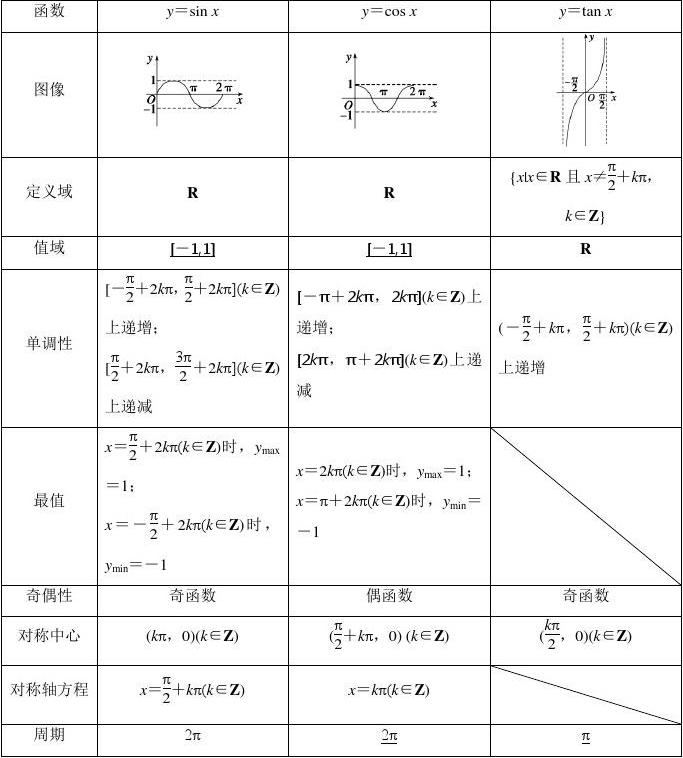
\includegraphics[scale=0.7]  {pic/sanjiaohanshu/sanjiaohanshuxingzhi.jpg}

\end{center}
%=========== 终边一点 ===========================================
\newpage
\subsection{终边一点}
{\color{red} 角$\alpha$ 终边上一点(-4,3):} \\
$\cos \alpha=\frac{x}{r}=\frac{x}{\sqrt{x^{2}+y^{2}}}=\frac{-4}{\sqrt{(-4)^{2}+3^{2}}}=-\frac{4}{5}$ \\
$\sin \alpha=\frac{y}{r}=\frac{y}{\sqrt{x^{2}+y^{2}}}=\frac{3}{\sqrt{(-4)^{2}+3^{2}}}=\frac{3}{5}$

%=========== 平移================================================

\subsection{平移}
{\color{red}  $\sin \left(2 x+\frac{\pi}{3}\right)$ 移动变成 $\sin \left(2 x+\frac{\pi}{6}\right)$:} \\
1) 提括号:	$\sin \left[2\left(x+\frac{\pi}{6}\right)\right]$ \quad $\sin \left[2\left(x+\frac{\pi}{12}\right)\right]$ \\
2) 相减:$\left(x+\frac{\pi}{12}\right)-\left(x+\frac{\pi}{6}\right)=-\frac{\pi}{12}$ \\
3) 翻译: $-\frac{\pi}{12}$ 是 向右移动 $\frac{\pi}{12}$

%=========== sin和cos 互化 =======================================

\subsection {sin和cos 互化}

$\cos \left(2 x+\frac{\pi}{3}\right) = sin\left(2 x+\frac{\pi}{3}+\frac{\pi}{2}\right)$  \quad 根据 $\cos x=\sin \left(x+\frac{\pi}{2}\right)$ \\
$\sin \left(2 x+\frac{\pi}{3}\right) = cos\left(2 x+\frac{\pi}{3}-\frac{\pi}{2}\right)$  \quad 根据 $\sin x=\cos \left(x-\frac{\pi}{2}\right)$

%=========== 区间内最值,值域=======================================

\subsection{区间内最值,值域}

%figure参数:h 此处(here)t 页顶(top)b 页底(bottom)p 独立一页(page)
\begin{minipage}[!h]{0.5\linewidth}
	{\color{red}   $f(x)=4 \sin \left(2 x-\frac{\pi}{3}\right)+\sqrt{3}$在$\left[0, \frac{\pi}{2}\right]$上的最大值,最小值 } \\
	$x \in\left[0, \frac{\pi}{2}\right]$ \\
	2$x \in[0, \pi]$ \\
	$2 x-\frac{\pi}{3} \in\left[-\frac{\pi}{3}, \frac{2}{3} \pi\right]$ \\
	如图此区间的最小值$-\frac{\sqrt{3}}{2}$,最大值1,所以 \\
	$ \sin\left(2 x-\frac{\pi}{3}\right) \in\left[-\frac{\sqrt{3}}{2}, 1\right]$ \\
	$4 \sin \left(2 x-\frac{\pi}{3}\right) \in[-2 \sqrt{3}, 4]$ \\
	$4 \sin \left(2 x-\frac{\pi}{3}\right)+\sqrt{3} \in[-\sqrt{3}, 4+\sqrt{3}]$
\end{minipage}
\hfill
\begin{minipage}[!h]{0.5\linewidth}
	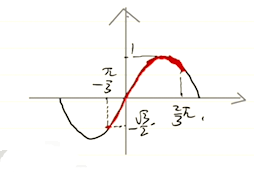
\includegraphics[scale=0.8]{pic/sanjiaohanshu/qujianneizuizhi.png}
\end{minipage}

%=========== 伸缩变换=============================================

\subsection {伸缩变换}
$y = \cos x$ \\
横坐标缩短到原来的$ \frac{1}{2} $ (x换成2x) $\longrightarrow$ $y= \cos 2x$ \\
纵坐标伸长到原来的2倍 (A换成2A) $\longrightarrow$ $y=  2 \cos 2x$ \\
向左平移 $\frac {\pi}{4} $  ($x$换成 $x+\frac{\pi}{4}$) $\longrightarrow$ $y=2 \cos \left[2\left(x+\frac{\pi}{4}\right)\right]$
%=========== 对称中心,对称轴,单调区间 =============================

\subsection {对称中心,对称轴,单调区间}

{\color{red}  $y=\sin \left(2 x-\frac{\pi}{3}\right)$ 的减区间} \\
\begin{figure}[h] %figure参数:h 此处(here)t 页顶(top)b 页底(bottom)p 独立一页(page)
	\begin{center}
		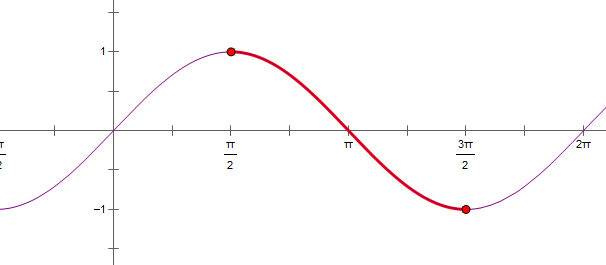
\includegraphics[scale=0.3]  {pic/sanjiaohanshu/dandiaojianqujian.png}
		\caption{$\sin x$ 减区间}
	\end{center}
\end{figure}


与基础图形对照:
\begin{tabular}{|c|c|}
	\hline
	$\sin x$ 减区间                              & $x \in\left[\frac{\pi}{2}+2 k \pi, \frac{3}{2} \pi+2 k \pi\right](k \in z)$                 \\
	\hline
	$\sin \left(2 x-\frac{\pi}{3}\right)$ 减区间 & $2 x-\frac{\pi}{3} \in\left[\frac{\pi}{2}+2 k \pi, \frac{3}{2} \pi+2 k \pi\right](k \in z)$ \\
	\hline
\end{tabular} \\
计算出$x$范围即可 . {\color{red}  对称中心,对称轴,同样原理,都是根据基础图形,替换即可}

%==============     sinx图像翻转 =================================
\subsection {sinx图像翻转}
$y=|\sin x|$ , $y=\sin |x|$ , $y=-\sin x$  \qquad (绿虚线:$\sin x$图像,红线:翻转后图像) \\
\begin{figure}[htbp]
	\begin{center}
		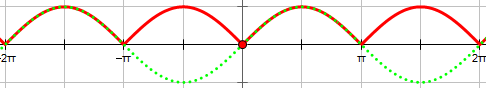
\includegraphics[scale=0.6]  {pic/sanjiaohanshu/abs(sin(x)).png}
		\caption{y=$|\sin x|$ $\qquad$ \textbf{整体加绝对值: x轴下方图像翻折到上方. 下方图像不保留.}  }
		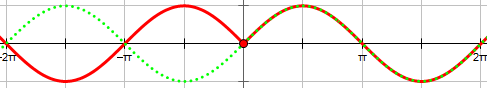
\includegraphics[scale=0.6]  {pic/sanjiaohanshu/sin(abs(x)).png}
		\caption{y=$\sin |x|$ $\qquad$\textbf{x加绝对值: 先画出 x 轴正半轴,再沿y轴翻折.}}
		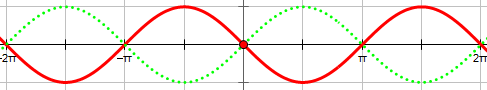
\includegraphics[scale=0.6]  {pic/sanjiaohanshu/-sinx.png}
		\caption{y=$-\sin x$ $\qquad$\textbf{整体加负号: 沿x轴上下翻折.}}
	\end{center}

\end{figure}

%==============     零点个数 =====================================
\subsection {零点个数}
{\color{red}  $f(x)=\left(\frac{1}{2}\right)^{x}-\sin x$ 在$[0,2\pi]$ 的零点个数} \\
令 $f(x)=0$ 即$\left(\frac{1}{2}\right)^{x}=\sin x$ \\
画出等号左右两侧图像,交点个数就是零点个数 (2个)
\begin{figure}[h] %figure参数:h 此处(here)t 页顶(top)b 页底(bottom)p 独立一页(page)
	\begin{center}
		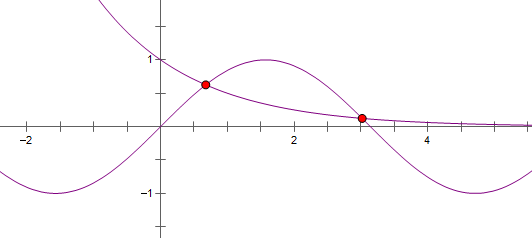
\includegraphics[scale=0.5]  {pic/sanjiaohanshu/lingdiangeshu.png}
		\caption{$f(x)=\left(\frac{1}{2}\right)^{x}$ , $f(x)=\sin x$}
	\end{center}
\end{figure}

\newpage
%==============  [ 正余弦 ]=======================================
\section{正余弦}
%==============  基础知识 ========================================
\subsection{基础知识}
{\color{blue} 正弦定理: } \\ $\frac{a}{\sin A}=\frac{b}{\sin B}=\frac{c}{\sin C}=2 R$ \\
{\color{blue}余弦定理: }\\ $a^{2}=b^{2}+c^{2}-2 b c \cos A \qquad b^{2}=a^{2}+c^{2}-2 a c \cos B \quad c^{2}=a^{2}+b^{2}-2 a b \cos C$ \\
\qquad \qquad $\cos A=\frac{b^{2}+c^{2}-a^{2}}{2 b c} \qquad \cos B=\frac{a^{2}+c^{2}-b^{2}}{2 a c} \qquad \cos C=\frac{a^{2}+b^{2}-c^{2}}{2 a b}$ \\
{\color{blue}面积公式:} \\
$S_{\Delta A B C}=\frac{1}{2} a b \sin C=\frac{1}{2} a c \sin B=\frac{1}{2} b c \sin A$ \\
$S=\frac{(a+b+c) r}{2}$ \qquad
$S=\frac{abc}{4R}$ \qquad $S=\sqrt{p(p-a)(p-b)(p-c)}$ \qquad ($p=\frac{1}{2}(a+b+c)$) \\
{\color{blue}判断三角形形状:}
最短两条边的平方与第三条边平方比较 \\
$a^{2}>b^{2}+c^{2} \quad \Delta A B C$ 为钝角三角形 \\
$a^{2}=b^{2}+c^{2} \quad \Delta A B C$ 为直角三角形 \\
$a^{2}<b^{2}+c^{2} \quad \Delta A B C$ 为锐角三角形 \\
%==============  多解取舍两种思路 ===============================
\subsection{多解取舍两种思路}
{\color{red} 在 $\Delta A B C$中,$b=\sqrt{3}, B=60^{\circ}, c=1$,求C } \\
$ \frac{b}{\sin B}=\frac{c}{\sin C} \therefore \sin C=\frac{1}{2} \therefore c=30^{\circ}$或$150^{\circ}$ \\
{\color{blue} 角度取舍两种思路: }\\
1) 依据大边对大角:  \quad
$\because b>c,  \therefore B>C \therefore C=30^{\circ}$ \\
2) 三角形内角和 $180^{\circ}$ : \quad
$ \because   B=60^{\circ}, \therefore 0^{\circ}<C<120^{\circ}  \therefore C=30^{\circ}$ \\

%============= 角化边,边化角,角化角 ===============================

\subsection{角化边,边化角}
{\color{red} $3a\cos A=c\cos B+b\cos C$,求$\cos A $} \\
两种思路都可以: \\
边 $\rightarrow$ 角 \\
$3 \sin A \cos A=\sin C \cos B+\sin B \cos C =\sin (B+C) =\sin A$
$\therefore   \cos A=\frac{1}{3}$ \\
角 $\rightarrow$ 边	 \\
$3 a \cos A=c \cdot \frac{a^{2}+c^{2}-b^{2}}{2 a c}+b \cdot \frac{a^{2}+b^{2}-c^{2}}{2 a b}$
$\therefore  \cos A=\frac{1}{3}$ \\
\subsection{角化角}
 {\color{red} $\sin B \cdot \sin C=\cos ^{2} \frac{A}{2}$ ,三角形形状 }

解:{\color{blue} 当出现三个角时,考虑角化角.化简成两个角的关系.} \\
先降幂: $\sin B \cdot \sin C=\cos ^{2} \frac{A}{2}=\frac{\cos A+1}{2}$ \\
{\color{blue} A角化成B+C }: $\therefore 2 \sin B \cdot \sin C = \cos A+1 =\cos(B+C)+1$ \\
化简计算即可: \\
$\therefore 2 \sin B \cdot \sin C=-\cos B \cos C+\sin B \sin C+1$ \\
$\therefore \cos B \cos C+\sin B \sin C=\cos (B-C)=1$ \\
$\therefore B-C=0, B=C$ \\
$\therefore$ 等腰
%============= 判断三角形形状 =====================================

\subsection{三角形形状(讨论n种情况)}

\begin{figure}[htbp] %figure参数:h 此处(here)t 页顶(top)b 页底(bottom)p 独立一页(page)
	\centering
	\begin{minipage}{170pt}
		\centering
		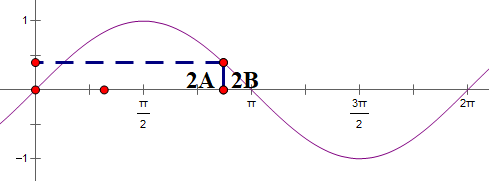
\includegraphics[width=170pt]  {pic/zhengyuxian/2A=2B.png}
		\caption{2A=2B}
	\end{minipage}
	\hspace{10pt}
	\begin{minipage}{170pt}
		\centering
		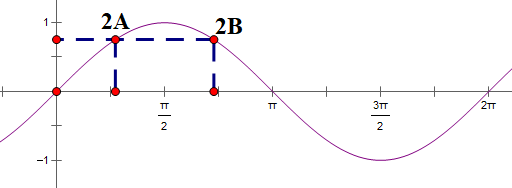
\includegraphics[width=170pt]  {pic/zhengyuxian/2A=2B1.png}
		\caption{$ 2A+2B= \frac{\pi}{2} * 2 $}
	\end{minipage}
	\hspace{10pt}
	\begin{minipage}{170pt}
		\centering
		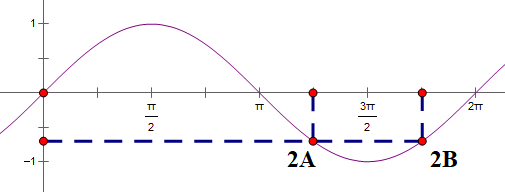
\includegraphics[width=170pt]  {pic/zhengyuxian/2A=2B2.png}
		\caption{$ 2A+2B= \frac{3\pi}{2} * 2 $}
	\end{minipage}
\end{figure}

{\color{red} $ \sin 2A= \sin 2B$ } \\

$\because 0<A<\pi \therefore 0<2A<2\pi$ \\
如图:三种情况 \\
1) 当$ 2A=2B $时 等腰三角形 \\
2) 当$ 2A+2B= \frac{\pi}{2} * 2 $ 时, 直角三角形 \\
3) 当$ 2A+2B= \frac{3\pi}{2} * 2 $ 时, 不符合三角形 \\




\subsection{已知三边判断三角形形状}
{\color{red} 已知三角形三边为 3,5,7 求三角形是形状(锐角,直角,钝角) } \\
$\because 3^{2}+5^{2}<7^{2}$ $\therefore$ 钝角


%============= [ 向量 ] ===========================================
\newpage
\section{向量}
%============= [ 基础知识 ] ========================================
\subsection{基础知识}


{\renewcommand\baselinestretch{2.5}\selectfont % 调整行间距
	\begin{tabular}{|c|c|c|}
		\hline
		                               & 线性运算                                                                                                                                          & 坐标运算                                                                                            \\
		\hline
		加法                           & \tabincell{c} {三角形法则:首尾相连首尾连: $\overrightarrow{A B}+\overrightarrow{B C}=\overrightarrow{A C}$                                                                                                                                              \\
		平行四边形法则:同起点,对角线 } & $\vec{a}+\vec{b}=\left(x_{1}+x_{2}, y_{1}+y_{2}\right)$                                                                                                                                                                                                 \\
		\hline
		减法                           & 三角形法则:同起点,连终点,指向被减向量:$\overrightarrow{A B}+\overrightarrow{A C}=\overrightarrow{C B}$                                          & $\vec{a}-\vec{b}=\left(x_{1}-x_{2}, y_{1}-y_{2}\right)$                                             \\
		\hline
		数乘                           & $x \vec{a}$ 表示与 $ \vec{a} $的方向相同($x>0$)或者相反($x<0$),长度为$\vec{a}$的$x$倍                                                             & $\lambda \vec{a}=\left(\lambda x_{1}, \lambda y_{1}\right)$                                         \\
		\hline
		数量积                         & $\vec{a} \cdot \vec{b}=|\vec{a}| \cdot|\vec{b}| \cos \theta$                                                                                      & $\vec{a} \cdot \vec{b}=x_{1} x_{2}+y_{1} y_{2}$                                                     \\
		\hline
		模                             & $|\vec{a} |=\sqrt{\vec{a}  \cdot \vec{a} }$ \qquad ($|\vec{a}|^{2}=\vec{a}^{2}$)                                                                  & $|\vec{a}|=\sqrt{x_{1}^{2}+y_{1}^{2}}$                                                              \\
		\hline
		夹角                           & $\cos \theta=\frac{\vec{a} \cdot \vec{b}}{|\vec{a}||\vec{b}|}$                                                                                    & $\cos \theta=\frac{x_{1} x_{2}+y_{1} y_{2}}{\sqrt{x_{1}^{2}+y_{1}^{2}} \sqrt{x_{2}^{2}+y_{2}^{2}}}$ \\
		\hline
		平行                           & $\vec{a}=\lambda \vec{b}(\vec{b} \neq 0)$                                                                                                         & $x_{1} y_{2}=x_{2} y_{1}$                                                                           \\
		\hline
		垂直                           & $\vec{a} \cdot \vec{b}=0$                                                                                                                         & $x_{1} x_{2}+y_{1} y_{2}=0$                                                                         \\
		\hline
		大写坐标                       & \multicolumn{2}{c}{ 设 $A\left(x_{1}, y_{1}\right), B\left(x_{2}, y_{2}\right)$ 则 $\overrightarrow{A B}=\left(x_{2}-x_{1}, y_{2}-y_{1}\right)$ }                                                                                                       \\
		\hline
	\end{tabular} \\
	\par}
%============= [ 绝对值 ] ==========================================

\subsection{绝对值}
{\color{red}  题目: } \\
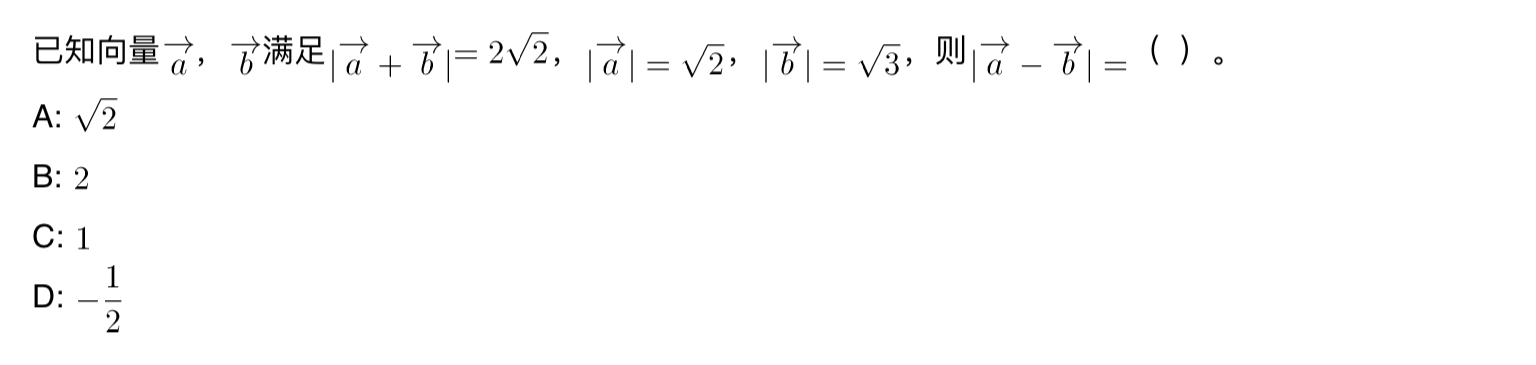
\includegraphics[width=500pt]  {pic/xiangliang/jueduizhi.jpg} \\
解: {\color{blue} 绝对值、想平方,算完之后不要慌. 因为算完后的 $\vec{a} \cdot \vec{b}$ 常常作为一个整体看待!}\\
$\because |\vec{a}+\vec{b}|^{2}=|\vec{a}|^{2}+|\vec{b}|^{2}+2 \vec{a} \cdot \vec{b}=8$ \\
$ \therefore 2 \vec{a} \cdot \vec{b}=3$ \\
$\therefore |\vec{a}-\vec{b}|^{2}=|\vec{a}|^{2}+|\vec{b}|^{2}-2 \vec{a} \cdot \vec{b}=2$ \\
$\therefore $ 选 A
%============= [ 夹角锐角钝角 ] =======================================

\subsection{夹角为锐角,钝角}
% {\color{blue} 绝对值、想平方,算完之后不要慌. }\\
{\color{red}  题目: } \\

\includegraphics[width=500pt]  {pic/xiangliang/jiajiaotimu.jpg} \\
解: {\color{blue}  $\vec{a} \cdot \vec{b}>0$ 且 不共线} \\
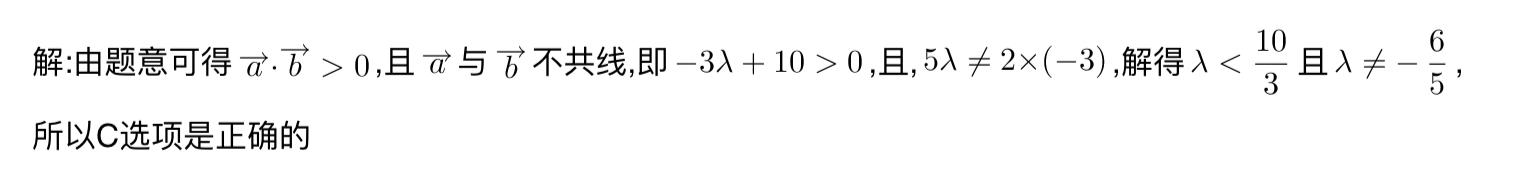
\includegraphics[width=500pt]  {pic/xiangliang/jiajiaojieda.jpg} \\

%============= [ 基础图形(理) ] ==========================================

\subsection{基础图形(理)}
{\color{red}  题目: } \\
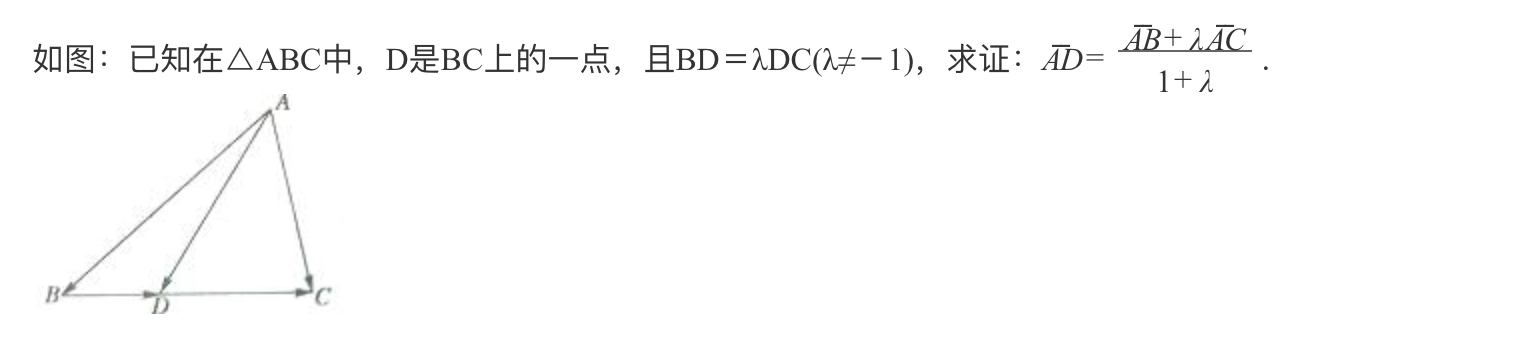
\includegraphics[width=500pt]  {pic/xiangliang/jichutuxingtimu.jpg}  \\
解: \\
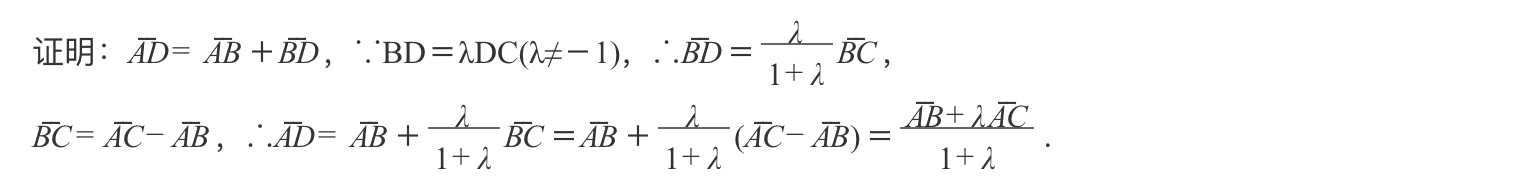
\includegraphics[width=500pt]  {pic/xiangliang/jichutuxingdaan.jpg} \\

%============= [ 基底建模法 ] ==========================================

\subsection{基底建模法(理)}
{\color{red}  题目: } \\
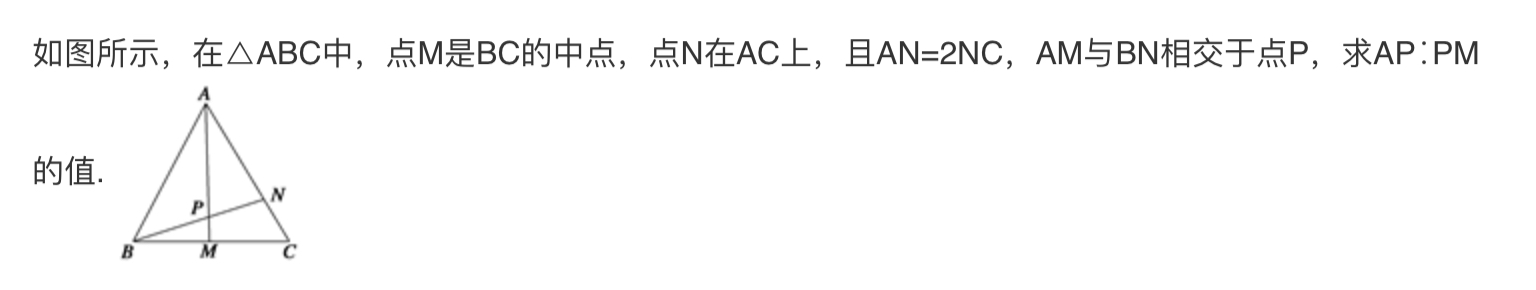
\includegraphics[width=500pt]  {pic/xiangliang/jidijianmofa.jpg} \\
解:{\color{blue} 以$\overrightarrow{B M}$,$\overrightarrow{C N}$为基底,进行计算.} \\
设:$e_{1}=\overrightarrow{B M}, \quad e_{2}=\overrightarrow{C N}$,则 \\ \\
$\overrightarrow{A M}=\overrightarrow{A C}+\overrightarrow{C M}=-3 e_{2}-e_{1}$ \\
$\overrightarrow{B N}=\overrightarrow{B C}+\overrightarrow{C N}=2 e_{1}+e_{2}$ \\
因为A,P,M和B,P,N分别共线 所以:\\ \\
$\overrightarrow{A P}=\lambda \overrightarrow{A M}=-\lambda e_{1}-$ 3$\lambda e_{2}$ \\
$\overrightarrow{B P}=\mu \overrightarrow{B N}=2 \mu e_{1}+\mu e_{2}$ \\ \\
$\overrightarrow{B A}=\overrightarrow{B P}-\overrightarrow{A P}=(\lambda+2 \mu) e_{1}+(3 \lambda+$ $\mu ) e_{2}$ \\
$\overrightarrow{B A}=\overrightarrow{B C}+\overrightarrow{C A}=2 e_{1}+3 e_{2}$ \\ \\
$\left\{\begin{array}{l}{\lambda+2 \mu=2} \\ {3 \lambda+\mu=3}\end{array}\right.$
$\left\{\begin{array}{l}{\lambda=\frac{4}{5}} \\ {\mu=\frac{3}{5}}\end{array}\right.$ \\
$\therefore A P : P M=4 : 1$


\newpage
%============= [ 数列 ] ==========================================
\section{数列}

%============= [ 基础知识 ] ======================================
\subsection{基础知识}
\begin{figure}[!h] %figure参数:h 此处(here)t 页顶(top)b 页底(bottom)p 独立一页(page)
	\centering
	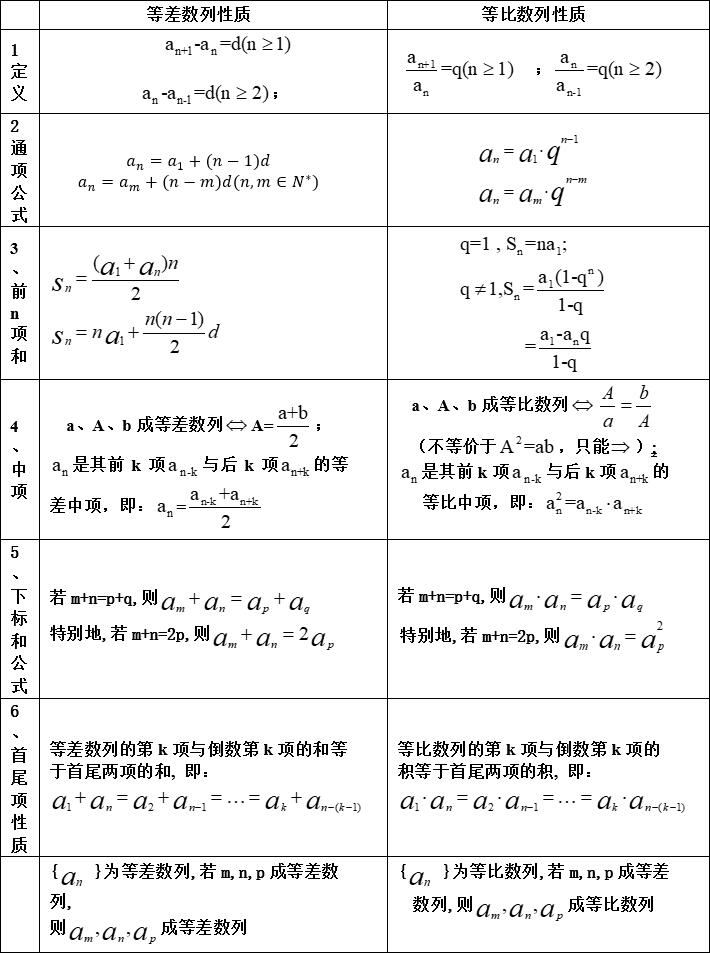
\includegraphics[width=450pt]  {pic/shulie/shuliexingzhi1.jpg} \\
\end{figure}
\begin{figure}[!h] %figure参数:h 此处(here)t 页顶(top)b 页底(bottom)p 独立一页(page)
	\centering
	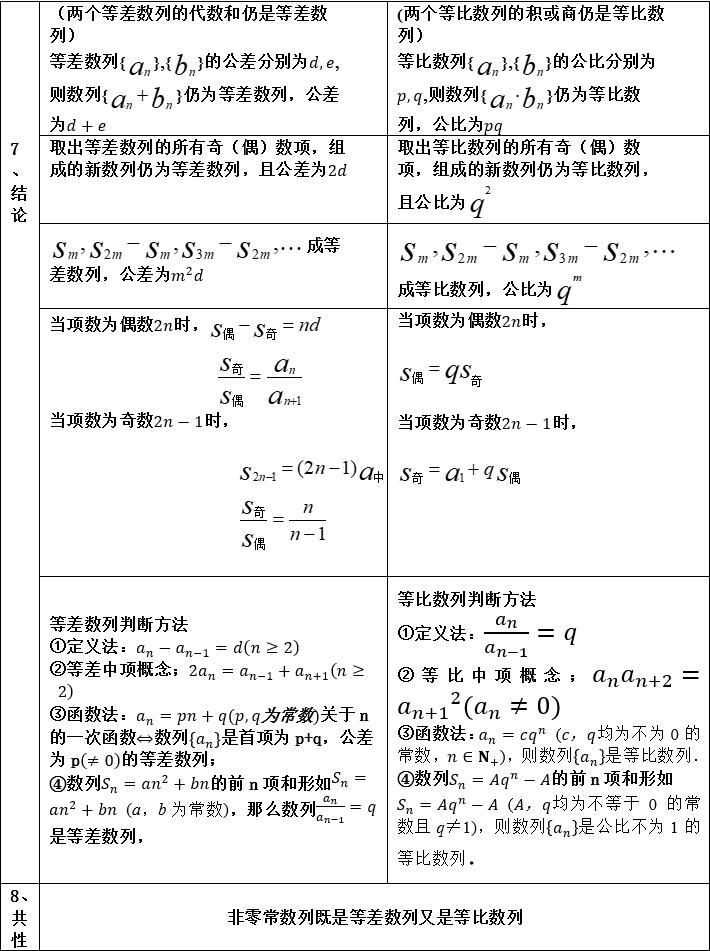
\includegraphics[width=450pt]  {pic/shulie/shuliexingzhi2.jpg} \\
\end{figure}

%============= [ 分式数列 ] ======================================
\clearpage
\subsection{单调性}
\subsubsection{分式数列}
{\color{red} 数列 $a_{n}=\frac{n-\sqrt{2016}}{n-\sqrt{2017}}$,则前100项的最大项,最小项是第几项 }\\
解: {\color{blue}  需要会分式函数的化简与图像: } \\
$a_{n}=\frac{n-\sqrt{2016}}{n-\sqrt{2017}}=1+\frac{\sqrt{2017}-\sqrt{2016}}{n-\sqrt{2017}}$ \\
根据函数图像: \\
当 $n \in[1,44]$ 时,$\left\{a_{n}\right\}$单调递减, \\
当 $n \in[45,+\infty)$ 单调递增, \\
$\therefore \left(a_{n}\right)_{\max }=a_{45},\left(a_{n}\right)_{\min }=a_{44}$

%============= [ 分段数列 ] ======================================

\subsubsection{分段数列}
{\color{red}  题目: } \\
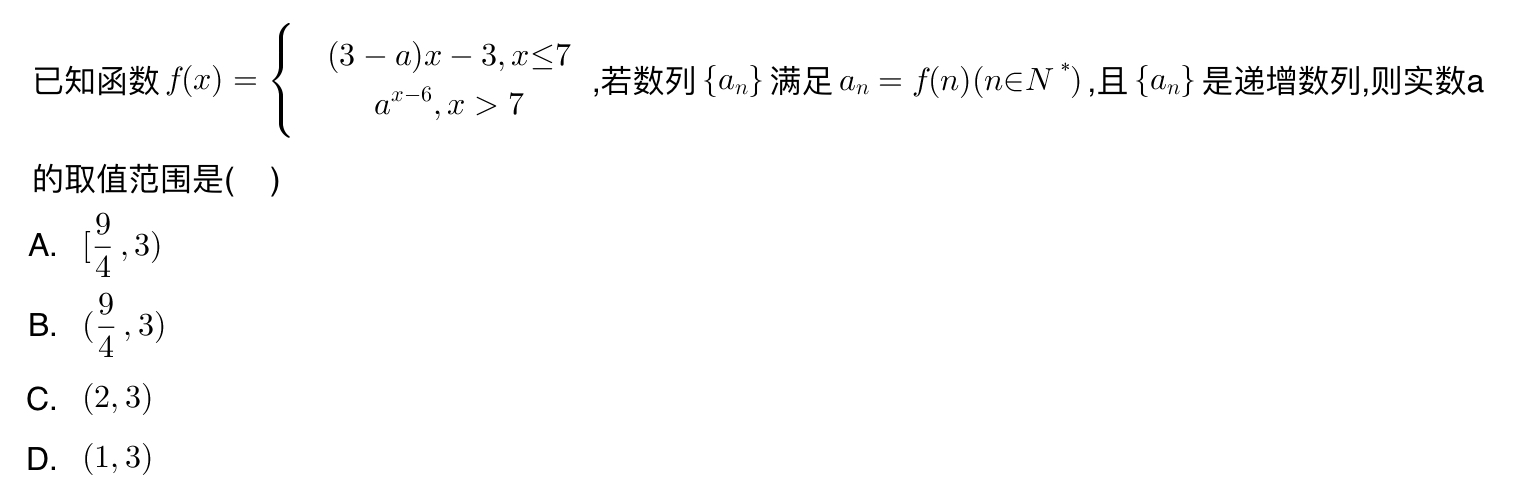
\includegraphics[width=500pt]  {pic/shulie/fenduanhanshutimu.jpg} \\
解: {\color{blue} 需要会分段函数单调性并注意与之对比: }\\
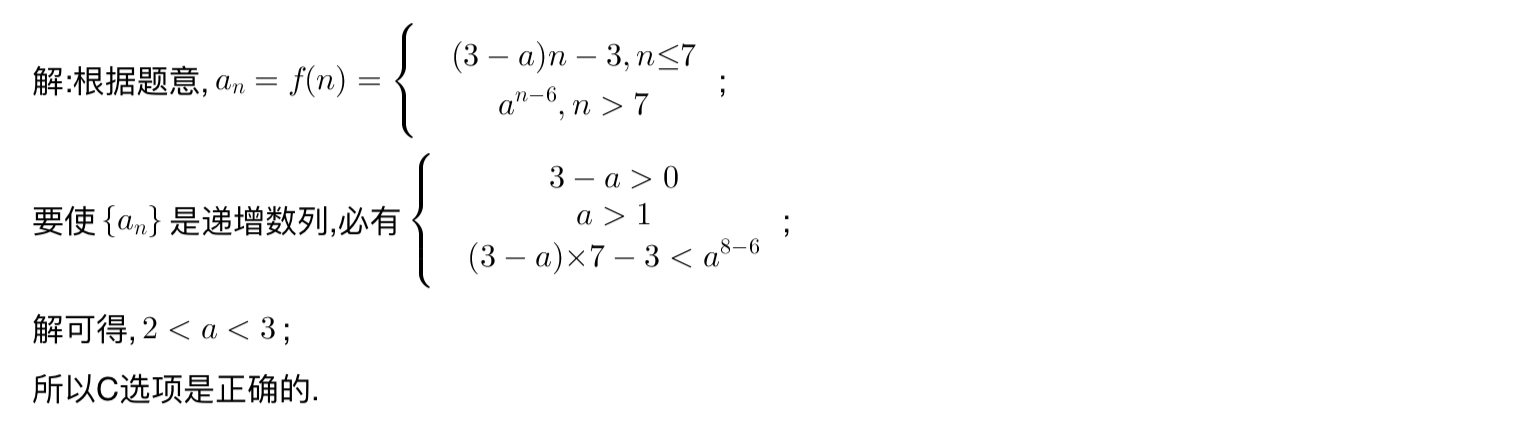
\includegraphics[width=500pt]  {pic/shulie/fenduanhanshudaan.jpg} \\

%============= [ 一般数列 ] ======================================

\subsubsection{一般数列}
{\color{red}  题目: } \\
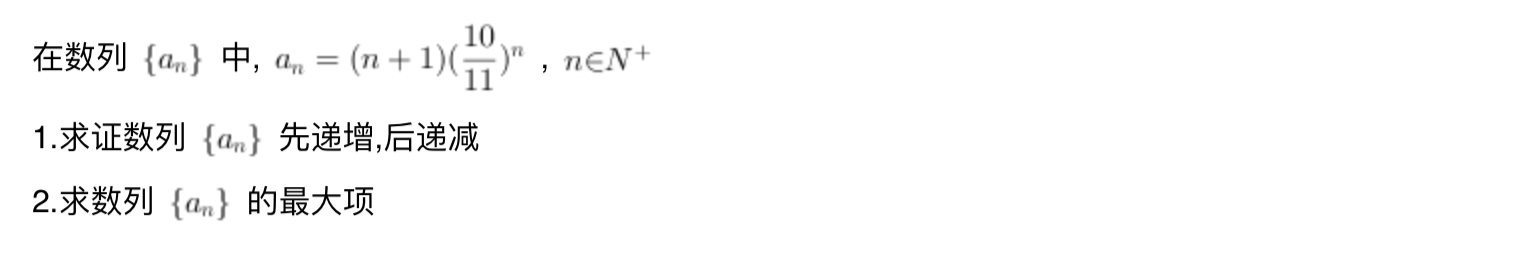
\includegraphics[width=500pt]  {pic/shulie/yibandandiaoxingtimu.jpg} \\
解: {\color{blue}  作差法或作商法: }\\
作差法: \\
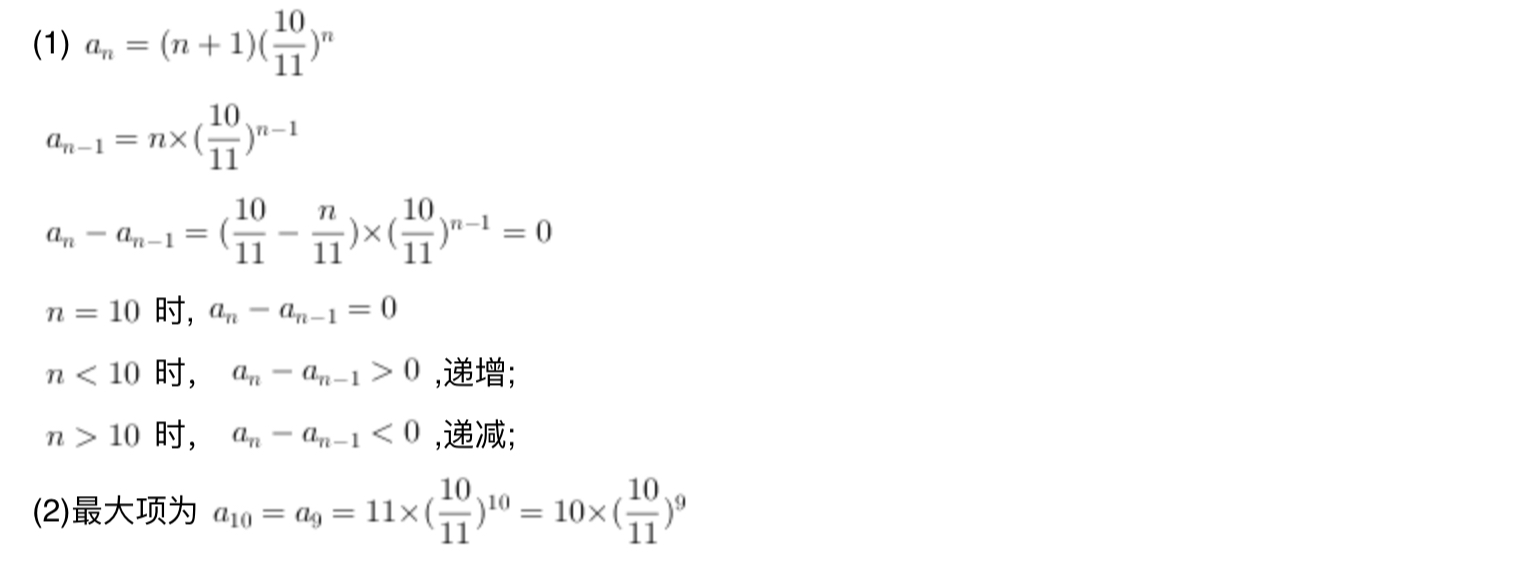
\includegraphics[width=500pt]  {pic/shulie/yibandandiaoxingdaan1.jpg} \\
作商法: \\
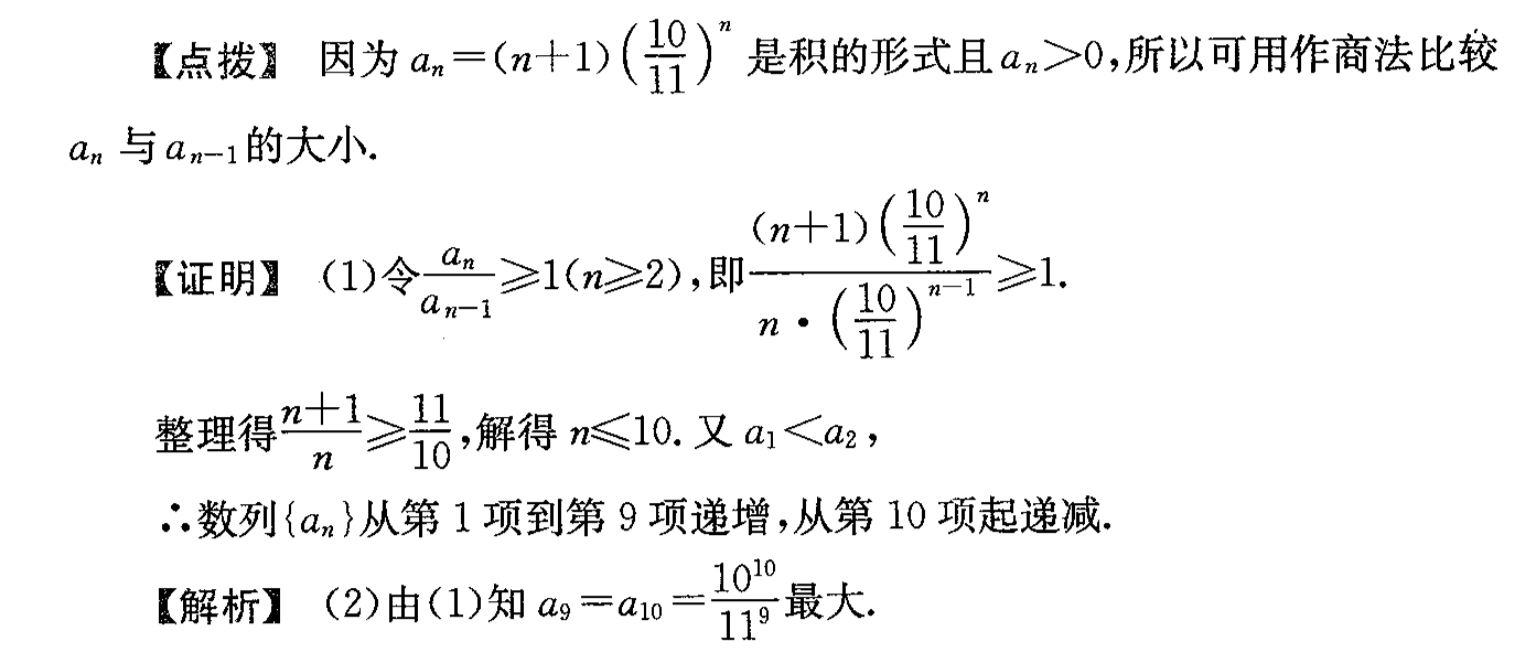
\includegraphics[width=350pt]  {pic/shulie/yibandandiaoxingdaan2.jpg} \\

%============= [ 最值 ] =========================================

\subsection{等差最值问题}
待补充
1.什么情况才会有最值? \\
2.最值的常见问法? \\
3.最值解题思路? \\
%============= [ 求通项公式 ] ====================================
\subsection{求通项公式 \texorpdfstring{$a_{n}$}{Lg}}

%============= [ Sn和n ] =========================================
\subsubsection{已知 \texorpdfstring{$S_{n}$}{Lg} 和\texorpdfstring{$n$}{Lg} 的关系,求\texorpdfstring{$a_{n}$}{Lg}   }
{\color{blue} 根据公式:$a_{n}=\left\{\begin{array}{ll}{S_{1}} & {(n=1)} \\ {S_{n}-S_{n-1}} & {(n \geqslant 2)}\end{array}\right.$ } \\
{\color{red}  $S_{n}=2 n^{2}+3 n+1$ ,求$a_{n}$} \\
解: \\
当n=1时,$a_{1}=S_{1}=6$ \\
当$n \geqslant 2$时,$a_{n}=S_{n}-S_{n-1}=4 n-1$ \\
({ \color{blue} 假设上式n=1,看是否也等于6,如果等于可以合在一块写.不等于要分段写.此题不等于. })\\
假设上式 n=1,则 $a_{1}=5\neq S_{1}$ \\
$ \therefore a_{n}=\left\{\begin{array}{ll}{6} & {n=1} \\ {4 n+1} & {n \geqslant 2}\end{array}\right.$
%============= [ Sn和an ] =========================================
\subsubsection{已知 \texorpdfstring{$S_{n}$}{Lg} 和\texorpdfstring{$a_{n}$}{Lg} 的关系,求\texorpdfstring{$a_{n}$}{Lg}   }

% \subsubsection{叠加法}
% 适用于:
% \subsubsection{叠乘法}
% 适用于:
% \subsubsection{倒数法}
% 适用于:
% \subsubsection{待定系数法}
% 适用于:
\subsection{求前n项和\texorpdfstring{$S_{n}$}{Lg}}
\subsubsection{裂项相消法}

如何裂项: $a_{n}=\frac{k}{b_{n} \cdot c_{n}}=\frac{k}{c_{n}-b_{n}}\left(\frac{1}{b_{n}}-\frac{1}{c_{n}}\right)$ \\
相消规律: 对称性 \\
最后结果尽量化简成1个分式 \\

例题: \\
{\color{red}求 $a_{n}=\frac{1}{(2 n-1)(2 n+1)}$前n项和 }\\
$a_{n}=\frac{1}{(2 n-1)(2 n+1)}=\frac{1}{2}\left(\frac{1}{2 n-1}-\frac{1}{2 n+1}\right)$ \\
$S_{n}=\frac{1}{2}\left(1-\frac{1}{3}+\frac{1}{3}-\frac{1}{5}+\frac{1}{5}-\frac{1}{7}+\cdots+\frac{1}{2 n-1}-\frac{1}{2 n+1}\right)$ \\
$=\frac{1}{2}\left(1-\frac{1}{2 n+1}\right)=\frac{n}{2 n+1}$ \\
\subsubsection{错位相减法}
适用于: 等差乘以等比 \\
步骤: 1.乘公比 2.错位 3.相减 \\
例题: \\
{\color{red} 求$a_{n}=n \cdot 2^{n}$的前n项和 }\\
$S_{n} =1 \cdot 2+2 \cdot 2^{2}+3 \cdot 2^{3}+\cdots+(n-1) \cdot 2^{n-1}+n \cdot 2^{n}$ \\
乘公比2 并错位写方便计算\\
$2 S_{n}=\qquad \quad 1 \cdot 2^{2}+2 \cdot 2^{3}+3 \cdot 2^{4}+\cdots+(n-1) \cdot 2^{n}+n \cdot 2^{n+1}$ \\
两式相减 \\
$-S_{n}=2+2^{2}+2^{3}+\dots+2^{n}-n \cdot 2^{n+1}$ \\
利用等比前n项和公式化简 \\
$S_{n}=(n-1) \cdot 2^{n+1}+2$
\end{document}
